
\section{Messungen an der Goldprobe}
 Die Goldprobe wird analog zur Graphitprobe in das Mikroskop eingelegt und angenähert. Anschließend werden die entsprechenden Parameter geladen: ein maximaler Tunnelstrom von $1\si{\nano\ampere}$ und eine Tunnelspannung von $100\si{\milli\ampere}$.

Da Gold als Leiter eine relativ homogene Elektronenverteilung besitzt, ist hier keine atomare Auflösung möglich. Wir beschränken uns deshalb auf die Topographie, die Spektroskopie und die 3D-Darstellung der Goldoberfläche.

\subsection{Topographie}
Wir wählten hier einen Scan-Bereich der Seitenlänge $105\si{\nano\meter}$, da ein übermäßiges Zoomen in die Probe, wie oben beschrieben, keinen Sinn macht. Nach nur wenigen Scan-Vorgängen konnten wir schon ein relativ schönes Bild der Goldoberfläche aufnehmen (siehe Abb. \ref{gold_oberfl}), die ein interessantes Höhenprofil aufweist. Dieses Bild kann nun auch genutzt werden, um die Stufenhöhe der Goldprobe zu ermitteln. Dazu wird eine Strecke auf der Oberfläche definiert, zu welcher man sich dann das Höhenprofil anzeigen lassen kann (siehe Abb. \ref{gold_profil}). Wir konnten somit eine Stufenhöhe von ca. $2\si{\angstrom}$ ermitteln, was mit dem Literaturwert von $2,36\si{\angstrom}$ vereinbar ist.

\subsection{Spektroskopie}
\paragraph{Strom-Spannungs-Kennlinie} Hier wurde im Spektroskopie-Modus die Tunnelspannung im Bereich von $-100\si{\milli\volt}$ bis $100\si{\milli\volt}$ variiert und der resultierende Tunnelstrom aufgetragen, siehe Abb. \ref{uigold} . Auch hier ist das erwartete lineare Verhalten, zwar etwas verrauscht, zu erkennen. Auch hier hält sich der maximale Tunnelstrom deutlich unter dem Grenzwert von $1\si{\nano\ampere}$.
\paragraph{Strom-Abstands-Kennlinie}
In Abb. \ref{uagold} ist die Strom-Abstands-Kennlinie zu sehen, wobei zu beachten ist, dass die y-Achse wieder logarithmisch skaliert ist. Diese Messung ist noch stärker verrauscht als bei Graphit, der exponentielle Zusammenhang lässt sich aber noch erahnen. Das starke Rauschen lässt sich eventuell durch die vergleichsweise  unebene Oberfläche der Goldprobe erklären.

\subsection{3D-Darstellung}
Analog zur Graphitmessung wurde mit der WSxM Software ein 3D-Bild der Goldoberfläche erstellt. Dieses ist in Abb. \ref{gold3d} zu sehen.

\begin{figure}[H]
	\begin{center}
	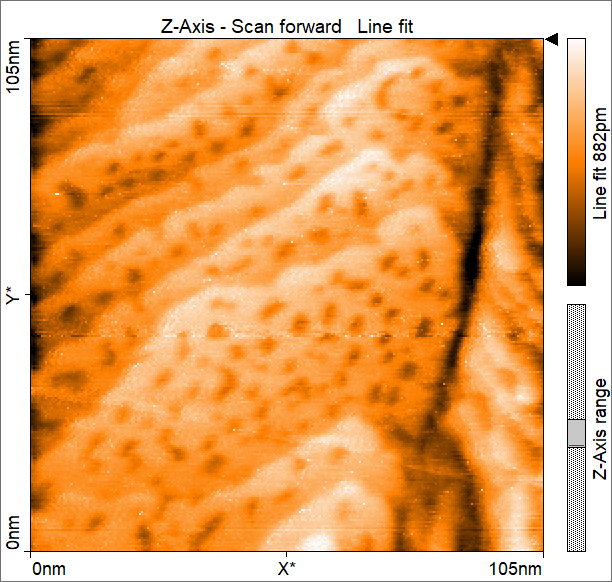
\includegraphics[width=10cm]{Mess/gold_oberfl.png}
	\caption{STM-Aufnahme der Goldoberfläche in einem Bereich mit 105nm Kantenlänge. Schön zu sehen ist das unebene Höhenprofil.}
	\label{gold_oberfl}
\end{center}
\end{figure}

\begin{figure}[H]
	\begin{center}
		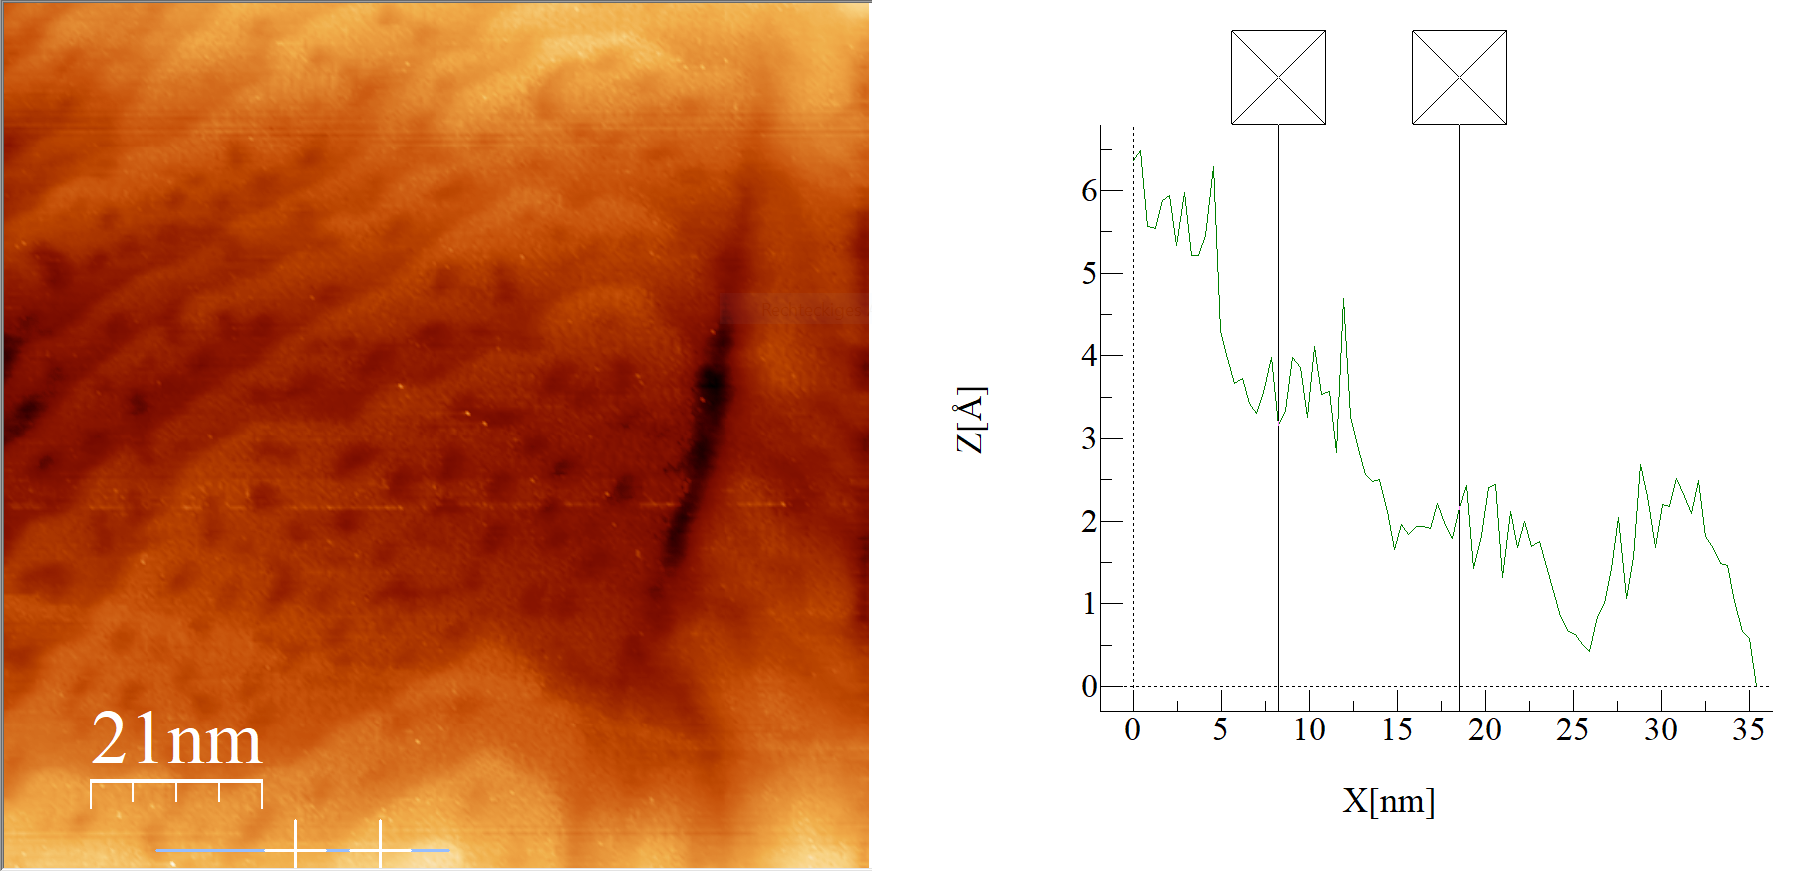
\includegraphics[width=\linewidth]{Mess/gold_profil.png}
		\caption{Messung der Stufenhöhe der Goldoberfläche. Hierzu wurde eine Strecke auf der Oberfläche ausgewählt (siehe linkes Bild, am unteren Rand) und dazu das Höhenprofil geplottet (rechtes Bild). Zu beachten ist, dass die Strecke von rechts nach links verläuft, das rechte Ende der Strecke also höher als das linke Ende liegt. Die Stufenhöhe beträgt ca. $2\si{\angstrom}$ bei einer geschätzten Unsicherheit von ca. $1\si{\angstrom}$.}
		\label{gold_profil}
	\end{center}
\end{figure}
	



\begin{figure}[H]
	\centering
	\begin{tikzpicture}
	\begin{axis}[
	xlabel={Spannung [mV]},
	ylabel={Tunnelstrom [pA]},
	%xmin=25,xmax=200,
	/pgf/number format/1000 sep={},
	legend pos=north west
	]
	\addplot[ 
	color = black,
	mark  = none,
	thick
	] table [
	%x=verz,y=int,
	x expr=\thisrowno{0}*10^3,
	y expr=\thisrowno{1}*10^12
	]
	{Mess/goldui.plt};
	\addlegendentry{Messwerte}
	\end{axis}
	\end{tikzpicture} 
	\caption{Strom-Spannungskurve von Gold. Wie für einen elektrischen Leiter erwartet findet sich hier ein linearer Zusammenhang.}
	\label{uigold}
\end{figure}



\begin{figure}[H]
	\centering
	\begin{tikzpicture}
	\begin{axis}[
	xlabel={Abstand [nm]},
	ylabel={Tunnelstrom [nA]},
	%xmin=25,xmax=200,
	/pgf/number format/1000 sep={},
	ymode=log,
	legend pos=north west,
	ymin=10e-4
	]
	\addplot[ 
	color = black,
	mark  = none,
	thick
	] table [
	%x=verz,y=int,
	x expr=\thisrowno{0}*10^9,
	y expr=\thisrowno{1}*10^9
	]
	{Mess/golddi.plt};
	\addlegendentry{Messwerte}
	\end{axis}
	\end{tikzpicture} 
	\caption{Strom-Abstands Kennlinie von Gold logarithmisch aufgetragen. Leider stark verrauscht, ab 39,2nm lässt sich noch ein linearer Abschnitt erahnen, was dem erwarteten exponentiellen Zusammenhang entspricht.}
	\label{uagold}
\end{figure}



\begin{figure}[H]
	\begin{center}
		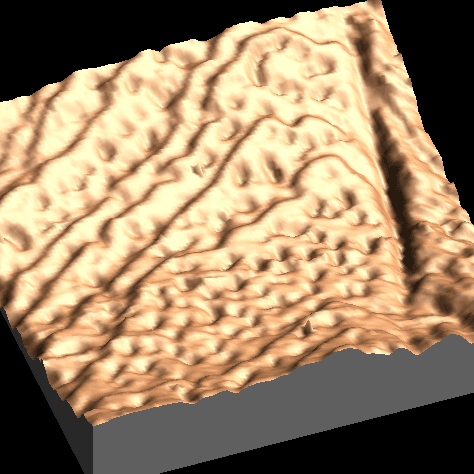
\includegraphics[width=9cm]{Mess/gold3d.png}
		\caption{3D-Darstellung der Goldoberfläche. Hier lässt sich das Oberflächenprofil besonders gut betrachten.}
		\label{gold3d}
	\end{center}
\end{figure}


\section{Messungen an der Molybdänsulfidprobe}

Bei der Molybdänsulfidprobe konnten trotz mehrmaliger Versuche bei verschiedenen Scan-Bereichen keine brauchbaren Aufnahmen der Oberfläche gemacht werden. Sämtliche Messungen resultierten in einem der Abb. \ref{mos_oberfl} ähnlichen Bild. Lediglich die Spektroskopie konnte mit akzeptablen Resultaten durchgeführt werden.

Die schlechte Qualität der Aufnahmen liegt vermutlich daran, dass die Spitze mit der Zeit unbrauchbar geworden ist (die Messung am Molybdänsulfit wurde zum Schluss durchgeführt) oder dass die Spitze einzelne Atome von der Probenoberfläche aufgenommen hat bzw. beim Scannen mitgezogen hat, was durchaus vorkommen kann. Manchmal hilft es hierbei, das Mikroskop einige Minuten lang scannen zu lassen, in der Hoffnung, dass sich die Spitze wieder stabilisiert. Leider blieb bei uns auch dieses Vorgehen ohne Erfolg.

\subsection{Spektroskopie}
\paragraph{Strom-Spannungs-Kennlinie}
Die Spannung wurde hier in einem Bereich von $-400\si{\milli\volt}$ bis $200\si{\milli\volt}$ variiert.
Da es sich bei Molybdänsulfit um einen Halbleiter handelt, weicht die Strom-Spannungs-Kennlinie deutlich von den beiden vorangegangenen Proben ab und zeigt kein lineares Verhalten (siehe Abb. \ref{uimos}). Stattdessen ist die Tunnelspannung bei niedrigen Spannungen nahezu konstant Null und steigt erst bei höheren Spannungen stark an, wie bei einem Halbleiter zu erwarten war.
\paragraph{Strom-Abstands-Kennlinie}
Die Strom-Abstands-Kennlinie (siehe Abb. \ref{uamos}) sieht auf den ersten Blick ebenfalls anders aus, als bei der Gold- oder Graphitprobe und ist bei hohen Abständen stark verrauscht. Bei genauerem Betrachten kann man jedoch erkennen, dass der Tunnelstrom bei Verringern des Abstandes auch exponentiell steigt und die Kurve erst ab ca. $1,5\si{\nano\ampere}$ (das ist der Grenzwert für die Tunnelspannung bei MoS2!) abflacht. Innerhalb der Grenzwerte lässt sich hier also ebenfalls ein exponentielles Verhalten beobachten.

\begin{figure}[H]
	\begin{center}
		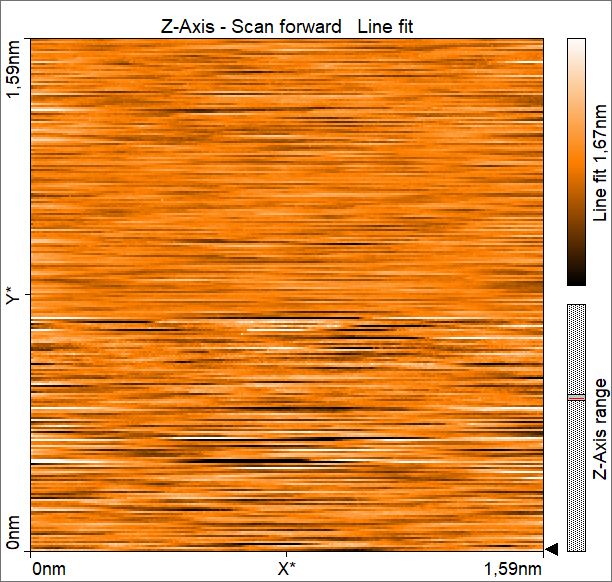
\includegraphics[width=10cm]{Mess/mos_oberfl.png}
		\caption{Fehlgeschlagene Messung der Molybdänsulfidprobe, es sind keine Strukturen erkennbar.}
		\label{mos_oberfl}
	\end{center}
\end{figure} 



\begin{figure}[H]
	\centering
	\begin{tikzpicture}
	\begin{axis}[
	xlabel={Spannung [mV]},
	ylabel={Tunnelstrom [pA]},
	%xmin=25,xmax=200,
	/pgf/number format/1000 sep={},
	legend pos=north west
	]
	\addplot[ 
	color = black,
	mark  = none,
	thick
	] table [
	%x=verz,y=int,
	x expr=\thisrowno{0}*10^3,
	y expr=\thisrowno{1}*10^12
	]
	{Mess/mosui.plt};
	\addlegendentry{Messwerte}
	\end{axis}
	\end{tikzpicture} 
	\caption{Strom-Spannungskurve von Molybdänsulfid. Hier zeigt sich, wie erwartet, kein linearer Zusammenhang, sondern ein typisches Halbleiterverhalten.}
	\label{uimos}
\end{figure}




\begin{figure}[H]
	\centering
	\begin{tikzpicture}
	\begin{axis}[
	xlabel={Abstand [nm]},
	ylabel={Tunnelstrom [pA]},
	%xmin=25,xmax=200,
	/pgf/number format/1000 sep={},
	ymode=log,
	legend pos=north west
	]
	\addplot[ 
	color = black,
	mark  = none,
	thick
	] table [
	%x=verz,y=int,
	x expr=\thisrowno{0}*10^9,
	y expr=\thisrowno{1}*10^12
	]
	{Mess/mosdi.plt};
	\addlegendentry{Messwerte}
	\end{axis}
	\end{tikzpicture} 
	\caption{Strom-Abstandskurve von Molybdänsulfid. Ab ca. -37nm beginnt ein linearer Abschnitt, der jedoch bei Erreichen des Grenzwertes für die Tunnelspannung von 1,5nA wieder abflacht.}
	\label{uamos}
\end{figure}

\chapter{Fazit}
Der Versuch dient als gute Einführung in die Thematik der Rastersondenmikroskopie. Neben den theoretischen Kenntnissen, die in der Vorbereitung erworben werden, erhält man auch schöne Einblicke in die Praxis der Rastertunnelmikroskopie, insbesondere auch in die Fehlerbehebung, welche von mehrmaligen Scannen in der Hoffnung auf Besserung, über Auswahl einer anderen Stelle auf der Probe bis hin zum Austausch der Spitze (inklusive deren Herstellung aus einem Draht) reicht. Schon bei diesem einfachen Versuchsaufbau wird deutlich, wie viel Aufwand unter Umständen betrieben werden muss, um ein akzeptables Bild zu erhalten, aus dem brauchbare Information gewonnen werden kann und lässt erahnen, wie schwer dies bei komplexeren Messungen sein kann.

Die Möglichkeit, selbst Aufnahmen mit nahezu atomarer Auflösung zu machen und diese stets verbessern zu wollen, stellt sich als interessantes Forschungsgebiet in der Physik heraus und dient als schöne Fortführung zum AFM-Versuch aus dem F1-Praktikum, falls dieses absolviert wurde.

